\noindent\begin{minipage}{7cm}
\begin{description}
\item[Objectif :] comprendre l'instruction d'af\-fec\-ta\-tion en informatique.
\item[Syntaxe \python :] \mbox{}
	\begin{itemize}
	\item \texttt{variable = constante}
	\item \texttt{variable = expression}
	\end{itemize}
\end{description}
\end{minipage}
\mbox{}\hfill
\begin{tabular}{c}
%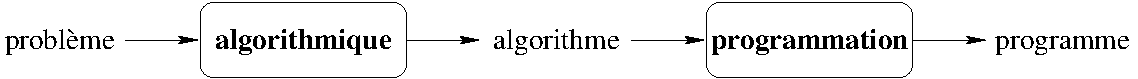
\includegraphics[width=8cm]{informatique-paysage.pdf}
\end{tabular}

%-------------------------------------------------------------------------
\subsection{Exemple}
%-------------------------------------------------------------------------

\noindent\begin{minipage}{9cm}
\paragraph{Objectif :} 
on veut ranger des objets de différents types dans un meuble à tiroirs
pour pouvoir les retrouver ultérieurement.
\vspace*{2mm}

\paragraph{Méthode :} 
proposer un mode de désignation des tiroirs qui permettra à une tierce
personne de retrouver sans ambiguïté les objets recherchés.

\end{minipage}
\hfill
\begin{minipage}{5cm}
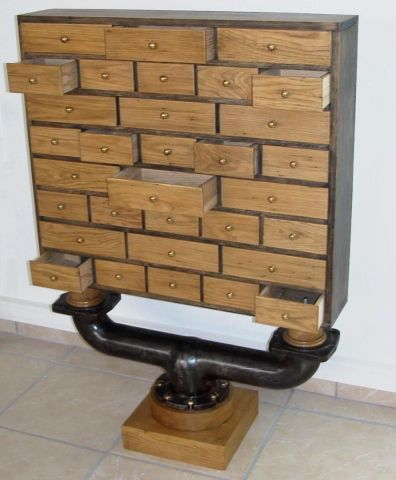
\includegraphics[width=4cm]{meuble.jpg}
\end{minipage}



\paragraph{Question :} 

\begin{question}[«~meuble à tiroirs~» : désignation des tiroirs]
Proposer un mode de désignation des tiroirs qui permette de retrouver
les objets.
\end{question}

\begin{question}[«~meuble à tiroirs~» : échange de contenus]
Utiliser ce mode de désignation pour expliquer comment échanger les contenus de deux tiroirs.
\end{question}

%-------------------------------------------------------------------------
\subsection{Généralisation}
%-------------------------------------------------------------------------
Une variable est un objet informatique qui associe un nom à une valeur 
qui peut éventuellement varier au cours du temps.
Une variable peut être vue comme une case en mémoire vive, que le programme 
va repérer par une étiquette (une adresse ou un nom). Pour avoir accès au contenu de la case
(la valeur de la variable), il suffit de la désigner par son étiquette : c'est-à-dire 
soit par son adresse en mémoire, soit par son nom.

\begin{question}[affectation : nommer les variables]
Dans l'exemple du «~meuble à tiroirs~», les tiroirs ont-ils un nom ?
Si oui, ce nom se réfère-t-il à son contenu (ie. a-t-on une idée du contenu d'un tiroir
rien qu'en connaissant son nom ?) ?
\end{question}


L'affectation est l'opération qui consiste à attribuer une valeur à une variable.

\begin{question}[affectation : constantes]
Donner quelques exemples de constantes possibles que l'on peut affecter à une variable.
\end{question}

\begin{question}[affectation : expressions]
Donner quelques exemples d'expressions possibles que l'on peut affecter à une variable.
\end{question}

\begin{question}[affectation : incrémentation]
Donner un exemple d'incrémentation d'une variable.
\end{question}

\begin{question}[affectation : égalité mathématique ?]
Montrer sur un exemple simple que l'affecta\-tion informatique est une opération différente de l'égalité mathématique.
\end{question}

\begin{question}[affectation : opération commutative ?]
Montrer sur un exemple simple que l'affec\-tation n'est pas commutative.
\end{question}

\begin{question}[affectation : fonctionnement]
Décrire l'exécution d'une instruction d'affectation.
\end{question}

L'affectation a ainsi pour effet de réaliser plusieurs opérations dans la mémoire de l'ordinateur :
\begin{itemize}
\item créer et mémoriser un nom de variable,
\item lui attribuer un type bien déterminé,
\item créer et mémoriser une valeur particulière,
\item établir un lien (par un système interne de pointeurs) entre le nom de la variable 
	et l'emplacement mémoire de la valeur correspondante.
\end{itemize}

%-------------------------------------------------------------------------
\subsection{Applications}
%-------------------------------------------------------------------------
\begin{question}[unité de longueur]
L'année-lumière (al) est une unité de distance utilisée en astronomie. 
Une année-lumière est la distance parcourue par un photon (ou plus simplement la lumière) 
dans le vide, en dehors de tout champ gravitationnel ou magnétique, en une année julienne 
(365,25 jours). 

Ecrire une instruction qui permette de passer directement des années-lumière aux $m$ sachant que
la vitesse de la lumière dans le vide est de 299 792 458 m/s.
\end{question}

\begin{question}[permutation circulaire]
Effectuer une permutation circulaire gauche entre les valeurs de 3 entiers $x$, $y$ et $z$.
\end{question}

\begin{question}[exécution d'une séquence d'affectations]
Quelles sont les valeurs des variables $a$, $b$, $q$ et $r$ après les séquences d'affectations suivantes ?

\begin{minipage}[t]{7cm}\em 
\begin{Verbatim}
a = 12 
b = 18
r = a%b
a = b
b = r
r = a%b
a = b
b = r
r = a%b
a = b
b = r
\end{Verbatim}
\end{minipage}
\hfill
\begin{minipage}[t]{7cm}\em 
\begin{Verbatim}
a = 19
b = 6
q = 0
r = a
r = r - b
q = q + 1
r = r - b
q = q + 1
r = r - b
q = q + 1
\end{Verbatim}
\end{minipage}


\end{question}


%-------------------------------------------------------------------------
%\newpage
\subsection{Entraînement}
%-------------------------------------------------------------------------

%-------------------------------------------------------------------------
\subsubsection{Enoncé}
%-------------------------------------------------------------------------
\paragraph{Contexte :} Le système international d'unités (\si) en physique est 
composé de 7 unités de base et de 2 unités supplémentaires définies dans le
tableau ci-dessous :
{\footnotesize
$$\begin{tabular}{|l|l|c|}
\hline
\textbf{Grandeur} & \textbf{Unité} & \textbf{Symbole}\\ 
\hline 
longueur						& mètre			& m \\ 
masse 							& kilogramme	& kg \\ 
temps							& seconde		& s \\ 
intensité de courant électrique & ampère		& A \\ 
température thermodynamique 	& kelvin		& K \\ 
quantité de matière 			& mole			& mol \\ 
intensité lumineuse 			& candela		& cd \\ 
\hline 
angle plan 						& radian		& rad \\ 
angle solide					& stéradian		& sr \\ 
\hline 
\end{tabular}$$}

\noindent Pour des raisons historiques, culturelles ou pragmatiques, un certain nombre 
d'unités hors-système, telles que l'heure (h), le grade (gr),
le pound (lb), le n\oe ud (kn), l'année-lumière (al) ou encore l'électronvolt (eV), 
peuvent être utilisées. Il est par contre nécessaire de connaître leur facteur 
de conversion en unités \si. Le tableau ci-dessous donne les facteurs de conversion
des unités les plus connues.
{\footnotesize
$$\begin{tabular}{|l|l@{ = }r@{ $\times$ }ll|l|}  
\hline
\bf Grandeur    & \multicolumn{4}{c|}{\textbf{Facteur de conversion}} & \textbf{Domaine} \\ 
\hline
année-lumière 	& 1 al 		& $9.46053$	& $10^{15}$ 	& $\textrm{m}$ 		& astronomie\\ 
atmosphère		& 1 atm 	& $1.01325$	& $10^{5}$  	& $\textrm{Pa}$ 	& météorologie \\
baril			& 1 b		& $0.15891$	& $10^{0}$		& $\textrm{m}^3$	& pétrole \\
calorie			& 1 cal		& $4.184$	& $10^{0}$		& $\textrm{J}$ 		& thermique \\
cheval-vapeur	& 1 ch		& $735.499$	& $10^{0}$		& $\textrm{W}$ 		& mécanique \\
curie			& 1 Ci		& $3.7$		& $10^{10}$ 	& $\textrm{Bq}$ 	& radioactivité \\
degré			& 1 $^\circ$& $1.745329$& $10^{-2}$   	& $\textrm{rad}$ 	& géométrie \\ 
électronvolt	& 1 eV		& $1.602189$& $10^{-19}$    & $\textrm{J}$ 		& physique nucléaire \\
faraday 		& 1 F		& $9.64870$	& $10^{4}$		& $\textrm{C}$ 		& électricité \\ 
foot			& 1 ft		& $30.48$	& $10^{-2}$		& $\textrm{m}$ 		& géométrie \\
franklin		& 1 Fr		& $3.33564$	& $10^{-10}$	& $\textrm{C}$ 		& électricité \\
frigorie		& 1 fg		& $4.186$	& $10^{3}$		& $\textrm{J}$ 		& thermique \\ 
gallon			& 1 gal		& $3.78541$	& $10^{-3}$		& $\textrm{m}^3$	& volume \\
grade			& 1 gr		& $1.570796$& $10^{-2}$		& $\textrm{rad}$ 	& géométrie \\
heure			& 1 h		& $3.6$		& $10^{3}$		& $\textrm{s}$ 		& temps \\
inch			& 1 in		& $2.54$	& $10^{-2}$		& $\textrm{m}$ 		& géométrie \\
lambert			& 1 L		& $3.183$	& $10^{3}$		& $\textrm{cd}\cdot\textrm{m}^{-2}$ 	& photométrie \\
mile			& 1 mile	& $1.609344$& $10^{3}$		& $\textrm{m}$ 		& géométrie \\ 
millimètre de mercure & 1 mmHg & $133.3224$ & $10^{0}$	& $\textrm{Pa}$ 	& météorologie \\
n\oe ud			& 1 nd		& $0.514444$& $10^{0}$		& $\textrm{m}\cdot\textrm{s}^{-1}$ 		& marine \\
oersted			& 1 Oe		& $79.57747$& $10^{0}$		& $\textrm{A}\cdot\textrm{m}^{-1}$ 		& magnétisme \\
parsec			& 1 pc		& $3.0857$	& $10^{16}$		& $\textrm{m}$ 		& astronomie\\ 
pica			& 1 pica	& $4.2175$	& $10^{-3}$		& $\textrm{m}$ 		& typographie\\ 
torr			& 1 Torr	& $133.3224$& $10^{0}$		& $\textrm{Pa}$		& météorologie \\
\hline
\end{tabular}$$ 
}

\paragraph{Objectif :} utiliser l'affectation pour calculer un facteur de conversion entre 
deux unités physiques comptatibles.

\paragraph{Méthode :} déterminer une relation entre les deux unités considérées en tenant 
compte de leur définition.

\paragraph{Vérification :} vérifier le bon fonctionnement sous \python{} en testant avec des valeurs remarquables connues.

%-------------------------------------------------------------------------
\subsubsection{Exemple}
%-------------------------------------------------------------------------
On veut convertir une température \bsc{Fahrenheit} en une température \bsc{Celsius}.
\begin{itemize}
\item La température \bsc{Celsius} $t_C$ (en $^\circ$C) est définie en fonction 
	de la température thermodynamique $T$ (en K) par la relation $t_C = T - 273.15$. 
\item La température \bsc{Fahrenheit} $t_F$ (en $^\circ$F) est définie en fonction 
	de la température thermodynamique $T$ (en K) par la relation $t_F = 9/5\cdot T - 459.67$. 
\end{itemize}

\paragraph{Méthode :} On cherche à exprimer $t_C$ (la température souhaitée)
en fonction de $t_F$ (la température donnée).
De la définition de $t_F$, on peut exprimer la température thermodynamique $T$
en fonction de la température \bsc{Fahrenheit} :\\
$T = 5/9\cdot(t_F + 459.67)$\\
On reporte l'expression de $T$ dans la définition de la température \bsc{Celsius} pour obtenir
une relation liant $t_C$ à $t_F$ :\\
$t_C = 5/9\cdot(t_F + 459.67) - 273.15$. 
\vspace*{2mm}

\noindent
\begin{minipage}[t]{7cm}
\paragraph{Résultat} En \python, une simple instruction d'affectation permet 
donc de passer de la température \bsc{Fahrenheit} initiale (\texttt{f}) à 
la température \bsc{Celsius} recherchée (\texttt{c}).

Pour la tester, on fixera $f$ à des valeurs connues : température de l'eau glacée 
($t_s = 32^{\circ}F$) et température de l'eau bouillante 
($t_g = 212^{\circ}F$), et on vérifiera qu'on obtient bien respectivement 
$c_s = 0^{\circ}C$ et $c_g = 100^{\circ}C$.
\end{minipage}
\hfill
\begin{minipage}[t]{8cm}
\begin{lstlisting}
c = 5/9*(f + 459.67) - 273.15
\end{lstlisting}
\end{minipage}

\paragraph{Vérification} on compare le résultat obtenu avec la valeur connue
de la température \bsc{Celsius}.
			
\begin{minipage}[t]{7cm}\footnotesize
température de l'eau glacée
\begin{Verbatim}
>>> f = 32
>>> c = 5/9*(f + 459.67) - 273.15
>>> c - 0
5.684341886080802e-14
\end{Verbatim}
\end{minipage}
\hfill
\begin{minipage}[t]{7cm}\footnotesize
température de l'eau bouillante
\begin{Verbatim}
>>> f = 212
>>> c = 5/9*(f + 459.67) - 273.15
>>> c - 100
5.684341886080802e-14
\end{Verbatim}
\end{minipage}
\vspace*{2mm}

\noindent
Les différences observées sont bien quasi-nulles ($10^{-14} \approx 0$).

%-------------------------------------------------------------------------
%\newpage
\subsubsection{Questions}
%-------------------------------------------------------------------------

Ecrire une affectation qui calcule les facteurs de conversion suivants.

\noindent\begin{minipage}[t]{7cm}
\begin{enumerate}
\item année-lumière en mile
\item année-lumière en parsec
\item parsec en foot
\item parsec en inch
\item parsec en année-lumière
\item inch en foot
\end{enumerate}
\end{minipage}
\hfill
\begin{minipage}[t]{7cm}
\begin{enumerate}\setcounter{enumi}{6}
\item inch en pica
\item foot en inch
\item centimètre en pica
\item mile en inch
\item mile en foot
\item année en minute
\end{enumerate}
\end{minipage}

\noindent\begin{minipage}[t]{7cm}
\begin{enumerate}\setcounter{enumi}{12}
\item année en seconde
\item baril en litre
\item baril en gallon
\item litre en gallon
\item litre en baril
\item électronvolt en calorie
\end{enumerate}
\end{minipage}
\hfill
\begin{minipage}[t]{7cm}
\begin{enumerate}\setcounter{enumi}{18}
\item électronvolt en frigorie
\item frigorie en calorie
\item franklin en faraday
\item n\oe ud en kilomètre par heure
\item torr en millimètre de mercure
\item atmosphère en torr
\end{enumerate}
\end{minipage}

%-------------------------------------------------------------------------
\subsection{Révisions}
%-------------------------------------------------------------------------

$$\begin{tabular}{|ll@{ : }l|}
\hline
\textbf{Cours} & \cite{cours} & chapitre 2, section 2.2 \\
\textbf{TD}    & \cite{td}    & exercices 2.1 à 2.4, 2.26 à 2.29 \\
\hline
\end{tabular}$$
